\documentclass[titlepage,landscape]{seminar}
\usepackage{url}
\usepackage{graphicx}
\usepackage{hyperref}
\usepackage{epstopdf}
\usepackage{slides}

\newcommand{\frack}{\frac{1}{k}}

\begin{document}

\myslide{
\heading{Genetic drift: Haploid population, $N=2$}
\begin{eqnarray*}
\mbox{Frequency of $A_1$ in parents} &=& p \\
\end{eqnarray*}
\vfill
}
\myslide{
\heading{Genetic drift: Haploid population, $N=2$}
\begin{eqnarray*}
\mbox{Frequency of $A_1$ in parents} &=& p \\
\mbox{Probability that both offspring are $A_1$} &=&  \\
\mbox{Probability that one offspring is $A_1$ and one is $A_2$} &=& \\
\mbox{Probability that both offspring are $A_2$} &=& 
\end{eqnarray*}
\vfill
}
\myslide{
\heading{Genetic drift: Haploid population, $N=2$}
\begin{eqnarray*}
\mbox{Frequency of $A_1$ in parents} &=& p \\
\mbox{Probability that both offspring are $A_1$} &=& p^2 \\
\mbox{Probability that one offspring is $A_1$ and one is $A_2$} &=& 2pq \\
\mbox{Probability that both offspring are $A_2$} &=& q^2
\end{eqnarray*}
\vfill
\begin{eqnarray*}
P(p'=1) &=& p^2  \\
P(p'=1/2) &=& 2pq \\
P(p'=0) &=& q^2 
\end{eqnarray*}
}

\myslide{
\heading{Genetic drift: Haploid population, $N=2$}
\begin{eqnarray*}
P(p_1=1|p_0) &=& p_0^2  \\
P(p_1=1/2|p_0) &=& 2p_0q_0 \\
P(p_1=0|p_0) &=& q_0^2  
\end{eqnarray*}
\vfil
\begin{eqnarray*}
P(p_2=1|p_1) &=& p_1^2 \\
P(p_2=1/2|p_1) &=& 2p_1q_1 \\
P(p_2=0|p_1) &=& q_1^2 
\end{eqnarray*}
}

\myslide{
\heading{Genetic drift: Haploid population, $N=2$}
\footnotesize
\begin{eqnarray*}
P(p_2=1|p_0) &=& P(p_2=1|p_1=1)P(p_1=1|p_0) + P(p_2=1|p_1=1/2)P(p_1=1/2|p_0) \\
             &=& (1)(p_0^2) + (1/4)(2p_0q_0) \\
             &=& p_0^2 + (1/2)p_0q_0 \\
P(p_2=1/2|p_0) &=& P(p_2=1/2|p_1=1/2)P(p_1=1/2|p_0) \\
               &=& (1/2)(2p_0q_0) \\
               &=& p_0q_0 \\
P(p_2=0|p_0) &=& P(p_2=0|p_1=0)P(p_1=0|p_0) + P(p_2=0|p_1=1/2)P(p_1=1/2|p_0) \\
             &=& (1)(q_0^2) + (1/4)(2p_0q_0) \\
             &=& q_0^2 + (1/2)p_0q_0 
\end{eqnarray*}
}

\myslide{
\heading{Genetic drift: Haploid population, $N=2$}
\footnotesize
\begin{eqnarray*}
P(p_2=1|p_0) &=& P(p_2=1|p_1=1)P(p_1=1|p_0) + P(p_2=1|p_1=1/2)P(p_1=1/2|p_0) \\
             &=& (1)(p_0^2) + (1/4)(2p_0q_0) \\
             &=& p_0^2 + (1/2)p_0q_0 \\
P(p_2=1/2|p_0) &=& P(p_2=1/2|p_1=1/2)P(p_1=1/2|p_0) \\
               &=& (1/2)(2p_0q_0) \\
               &=& p_0q_0 \\
P(p_2=0|p_0) &=& P(p_2=0|p_1=0)P(p_1=0|p_0) + P(p_2=0|p_1=1/2)P(p_1=1/2|p_0) \\
             &=& (1)(q_0^2) + (1/4)(2p_0q_0) \\
             &=& q_0^2 + (1/2)p_0q_0 \\
\end{eqnarray*}
}

\myslide{
\heading{Genetic drift: Haploid population, $N=2$}
\begin{eqnarray*}
P(p_t=1|p_0) &=& p_0^2 + \left(1 - (1/2)^{t-1}\right)p_0q_0 \\
P(p_t=1/2|p_0) &=& p_0q_0(1/2)^{t-2} \\
P(p_t=0|p_0) &=& q_0^2 + \left(1 - (1/2)^{t-1}\right)p_0q_0
\end{eqnarray*}
}


\myslide{
\heading{Genetic drift: Haploid population, $N=2$}
\begin{eqnarray*}
P(p_t=1|p_0) &=& p_0^2 + \left(1 - (1/2)^{t-1}\right)p_0q_0 \\
P(p_t=1/2|p_0) &=& p_0q_0(1/2)^{t-2} \\
P(p_t=0|p_0) &=& q_0^2 + \left(1 - (1/2)^{t-1}\right)p_0q_0 \\
\\
  \mbox{E}(p_t) &=& p_0^2 + \left(1 - (1/2)^{t-1}\right)p_pq_0
                    + p_0q_0 (1/2)^{t-2}(1/2) \\
             &=& p_0^2 + p_0q_0 \\
             &=& p_0(p_0 + q_0) \\
             &=& p_0
\end{eqnarray*}
}


\myslide{
\heading{Genetic drift: Diploid population, $N$ individuals}
\[
P(\hbox{$j$ $A_1$ in offspring $|$ $i$ $A_1$ in parents}) =
{2N \choose j}\left(\frac{i}{2N}\right)\left(1 - \frac{i}{2N}\right)
\]
\vfil
\[
\mbox{E}(p_t) = \frac{i}{2N}
\]
\vfil
\[
\hbox{Var}(p_{t+1}) = \frac{p_t(1-p_t)}{2N}
\]
}

\myslide{
\heading{Genetic drift: Analogy to inbreeding}
\begin{eqnarray*}
f_{t+1} &=& \mbox{Prob. ibd from preceding generation} + \\
        &&  (\mbox{Prob. not ibd from prec. gen.}) \times (\mbox{Prob. ibd from
          earlier gen.}) \\
\end{eqnarray*}
}

\myslide{
\heading{Genetic drift: Analogy to inbreeding}
\begin{eqnarray*}
f_{t+1} &=& \mbox{Prob. ibd from preceding generation} + \\
        &&  (\mbox{Prob. not ibd from prec. gen.}) \times (\mbox{Prob. ibd from
          earlier gen.}) \\
        && \\
        &=& \frac{1}{2N} + \left(1 - \frac{1}{2N}\right)f_t \\
\end{eqnarray*}
}

\myslide{
\heading{Genetic drift: Analogy to inbreeding}
\begin{eqnarray*}
f_{t+1} &=& \mbox{Prob. ibd from preceding generation} + \\
        &&  (\mbox{Prob. not ibd from prec. gen.}) \times (\mbox{Prob. ibd from
          earlier gen.}) \\
        && \\
        &=& \frac{1}{2N} + \left(1 - \frac{1}{2N}\right)f_t \\
  \\
f_{t+1} &=& 1 - \left(1 - \frac{1}{2N}\right)^t(1-f_0)
\end{eqnarray*}
}

\myslide{
\heading{Genetic drift: Variance effective size}
\[
Var(p_{t+1}) = \frac{p_t(1-p_t)}{2N} \quad.
\]
\vfil
\[
N_e^{(v)} = \frac{p(1-p)}{2\widehat{Var}(p)}
\]
}

\myslide{
\heading{Genetic drift: Inbreeding effective size}
\[
f_{t+1}
   = \frac{1}{2N} + \left(1 - \frac{1}{2N}\right)f_t
\]
\vfil
\[
N_e^{(f)} = \frac{1 - \hat f_t}{2(\hat f_{t+1} - \hat f_t)}
\]
\vfil
Assume $\hat f_t = 0$
\[
N_e^{(f)} = \frac{1}{2\hat f_{t+1}}
\]
}

\myslide{
\heading{Effective size: Variable population size}
\begin{eqnarray*}
f_{t+1} &=& \left(1-\frac{1}{2N_t}\right)f_t + \frac{1}{2N_t} \\
1 - f_{t+1} &=& \left(1-\frac{1}{2N_t}\right)(1-f_t) \\
1 - f_{t+K} &=&
\left(\prod_{i=1}^K\left(1-\frac{1}{2N_{t+i}}\right)\right)(1-f_t) \quad .
\end{eqnarray*}
}

\myslide{
\heading{Effective size: Variable population size}
\begin{eqnarray*}
f_{t+1} &=& \left(1-\frac{1}{2N_t}\right)f_t + \frac{1}{2N_t} \\
1 - f_{t+1} &=& \left(1-\frac{1}{2N_t}\right)(1-f_t) \\
1 - f_{t+K} &=&
\left(\prod_{i=1}^K\left(1-\frac{1}{2N_{t+i}}\right)\right)(1-f_t) \quad .
\end{eqnarray*}
If the population size were constant
\begin{eqnarray*}
\left(\prod_{i=1}^K\left(1-\frac{1}{2N_{t+i}}\right)\right) &=&
\left(1 - \frac{1}{2N_e^{(f)}}\right)^K \\
\sum_{i=1}^K\log\left(1-\frac{1}{2N_{t+i}}\right) &=&
K\log\left(1 - \frac{1}{2N_e^{(f)}}\right) 
\end{eqnarray*}
}

\myslide{
\heading{Effective size: Variable population size}

{\color{blue}\bf AWKF}: If $x$ is small, $\log(1 - x) \approx -x$
\begin{eqnarray*}
\sum_{i=1}^K\log\left(1-\frac{1}{2N_{t+i}}\right) &=&
K\log\left(1 - \frac{1}{2N_e^{(f)}}\right) \\
\sum_{i=1}^K-\frac{1}{2N_{t+i}}
  &\approx& K\left(-\frac{1}{2N_e^{(f)}}\right) \\
\frac{K}{N_e^{(f)}} &=& \sum_{i=1}^K\frac{1}{N_{t+i}} \\
\frac{1}{N_e^{(f)}} &=& \left(\frac{1}{K}\right)\sum_{i=1}^K\frac{1}{N_{t+i}} \\
N_e^{(f)} &=& \left(\left(\frac{1}{K}\right)
                    \sum_{i=1}^K\frac{1}{N_{t+i}}\right)^{-1}
\end{eqnarray*}
}

\myslide{
\heading{Effective size: Unequal sex ratio}
\begin{eqnarray*}
f_{t+1} &=& \left(\half\right) \left(\frac{N-1}{2N-1}\right)
            \left(\frac{1}{2N_f}\right) +
            \left(\half\right) \left(\frac{N-1}{2N-1}\right)
            \left(\frac{1}{2N_m}\right) \\
        &=& \left(\half\right) \left(\frac{N-1}{2N-1}\right)
            \left(\frac{1}{2N_f} + \frac{1}{2N_m}\right) \\
        &\approx& \left(\fourth\right)
            \left(\frac{2N_m + 2N_f}{4N_fN_m}\right) \\
        &=& \left(\half\right)
            \left(\frac{N_m + N_f}{4N_fN_m}\right) \\
N_e^{(f)} &\approx& \frac{4N_fN_m}{N_f + N_m} \quad 
\end{eqnarray*}
}

\myslide{
\heading{Effective size: Variance in offspring number}
\[
N_e^{(f)} = \frac{2N - 1}{1 + \frac{V_k}{2}} \quad ,
\]
\vfill
\begin{itemize}

\item $N_e^{(f)} < N$ if $V_k > 2(1 - 1/N)$ and

\item $N_e^{(f)} > N$ if $V_k < 2(1 - 1/N)$.

\end{itemize}
}

\myslide{
\heading{Drift and mutation}
\[
f_{t+1} = \left(\left(\frac{1}{2N}\right) +
          \left(1 - \frac{1}{2N}\right)f_t\right)(1-\mu)^2
\]
}

\myslide{
\heading{Drift and mutation}
\begin{eqnarray*}
\hat f &=& \left(\left(\frac{1}{2N}\right) +
          \left(1 - \frac{1}{2N}\right)\hat f\right)(1-\mu)^2 \\
\hat f\left(1 -
\left(1 - \frac{1}{2N}\right)(1-\mu)^2\right)
       &=& \left(\frac{1}{2N}\right)(1-\mu)^2 \\
\hat f &=& \frac{\left(\frac{1}{2N}\right)(1-\mu)^2}
           {1 -\left(1 - \frac{1}{2N}\right)(1-\mu)^2} \\
       &\approx& \frac{1 - 2\mu}
           {2N\left(1 - \left(1 - \frac{1}{2N}\right)(1-2\mu)\right)} \\
       &=& \frac{1 - 2\mu}
           {2N\left(1 - 1 + \frac{1}{2N} + 2\mu -
            \frac{2\mu}{2N}\right)} \\
       &=& \frac{1 - 2\mu}{1 + 4N\mu - 2\mu} \\
       &\approx& \frac{1}{4N\mu + 1}
\end{eqnarray*}
}

\myslide{
\heading{Drift and mutation}
\begin{center}
\resizebox{!}{0.9\textheight}{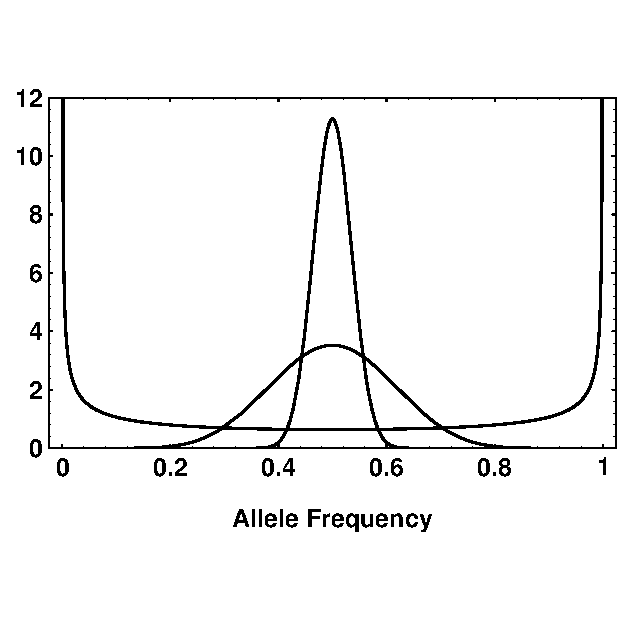
\includegraphics{mutation.eps}}
\end{center}
}

\myslide{
\heading{Drift and migration}
\[
f_{t+1} = \left(\left(\frac{1}{2N}\right) +
          \left(1 - \frac{1}{2N}\right)f_t\right)(1-m)^2
\]
\vfill
\[
\hat f \approx \frac{1}{4Nm + 1}
\]
}

\end{document}


